% !TeX root = ../main.tex

\chapter{引言}
\label{introduction}

  \section{研究背景}
  \label{introduction:background} 
  互联网自诞生以来,发展至今已成为重要的全球性信息化基础设施。在网络空间开展的人类活动日趋多样化,各种经济、政治、文化活动都经由互联网的传播而拥有了更为广泛的影响力,中国、美国等大国都针对网络空间制定了相应的发展战略\cite{china2016networkspace,USStrategyPlan}。

  但是,随着互联网的蓬勃发展,其最初的体系结构设计开始面临许多扩展性与安全性方面的新问题。

  首先,伴随着网络的普及,智能移动终端的飞速发展与物联网的兴起,接入互联网的设备数量发生了急剧的增长,网络中用于数据包路由寻址的网络层地址——IPv4地址\cite{RFC0791}遭遇了耗尽的问题。尽管互联网工程任务组(Internet Engineering Task Force,IETF)研制了许多方案试图增强IPv4地址的扩展能力,比如网络地址转换(Network Address Translation,NAT)\cite{RFC3022}和无类域间路由(Classless Inter-Domain Routing,CIDR)\cite{RFC1519}等,但也仅能推迟该问题的发生。由互联网号码分配局(Internet Assigned Numbers Authority,IANA)管理的IPv4地址已于2011年1月31日完全分配\cite{smith2011free},并且随着欧洲网络协调中心在2019年11月25日宣布其最后的IPv4地址空间耗尽\cite{RIPENCC},IPv4地址已经彻底枯竭。为了彻底解决IPv4地址枯竭的问题,必须将网络层的路由寻址切换至IPv6地址\cite{RFC2460}。相比于IPv4地址,IPv6地址拥有更为广阔的地址空间,并且其协议的设计也具有更加灵活的扩展性,因而使得在网络层添加和携带除路由信息以外的其他信息成为可能。IPv6地址作为网络体系结构中至关重要的网络层新标准,为各国发展下一代互联网技术提供了新的机遇,因而引起了世界各国政府的高度重视。近年来,IPv6在全球范围内的部署率如图\ref{fig:IPv6_deploy_trend}\footnote{https://www.google.com/intl/en/ipv6/statistics.html}所示,呈现明显上升的态势。

  \begin{figure}[ht]
    \centering
    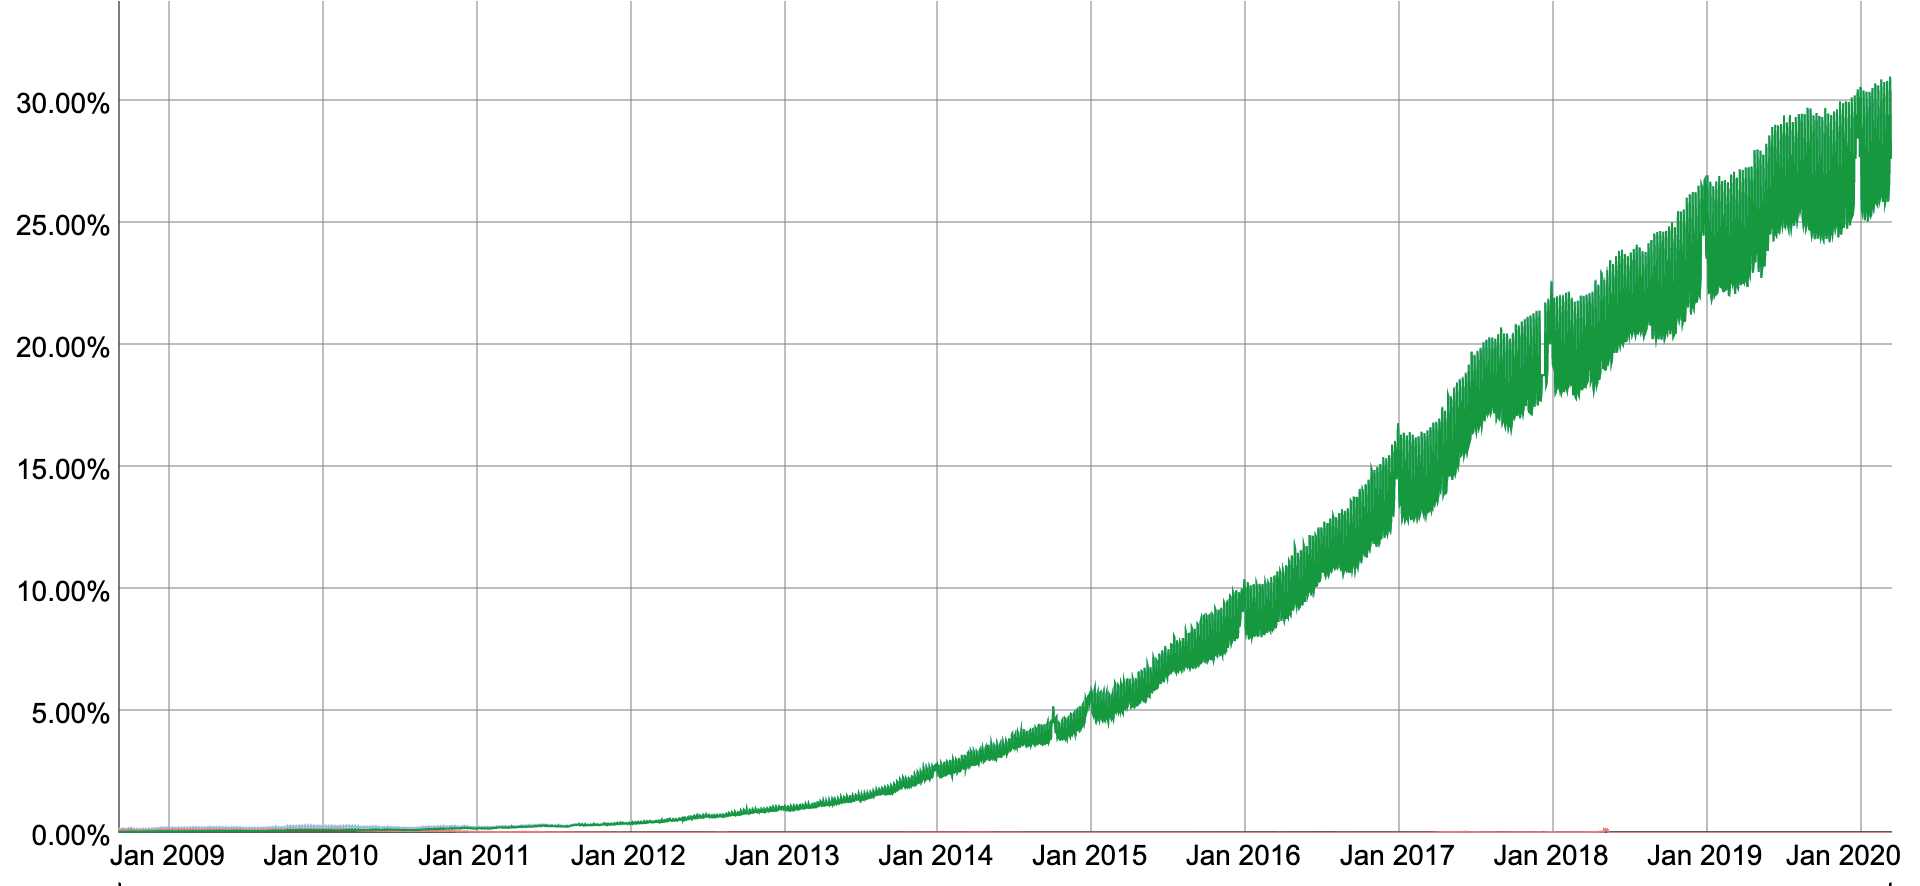
\includegraphics[width=0.9\textwidth]{IPv6_deploy_trend.png}
    \caption{IPv6部署率变化趋势}
    \label{fig:IPv6_deploy_trend}
  \end{figure}

  与此同时,由于互联网诞生之初的目标是成为美国内部学术机构和军事机构之间的连接设施,其假定了不存在恶意的参与者连接入网络,因而没有将网络的安全性作为最初设计时的主要目标之一。然而,随着互联网作为一项基础设施在全世界范围内得到广泛的应用,网络中恶意的攻击者层出不穷,网络体系结构设计中的安全问题也日益凸显。例如,分布式拒绝服务攻击(Distributed Denial of Service, DDoS)\cite{mirkovic2004taxonomy,douligeris2004ddos}至今仍在世界范围内广泛发生,每时每刻都在造成巨大的经济损失\cite{Kaspersky,DDosCost}。在美国白宫国家科技委员会网络和信息技术研发分委会发布的《网络安全研发战略规划》\cite{USStrategyPlan}中,网络安全的防御被分为四个主要阶段:威慑、保护、检测和适应,四者应对网络攻击时起效的顺序如图\ref{fig:security_methods}所示。可见,如果拥有强大的威慑手段,则很大一部分攻击者会因为攻击可能导致的后果而放弃发动攻击,而对于不惜代价发动的攻击行为,有效的保护手段则可以最大程度地减少攻击所带来的损失。
  \begin{figure}[ht]
    \centering
    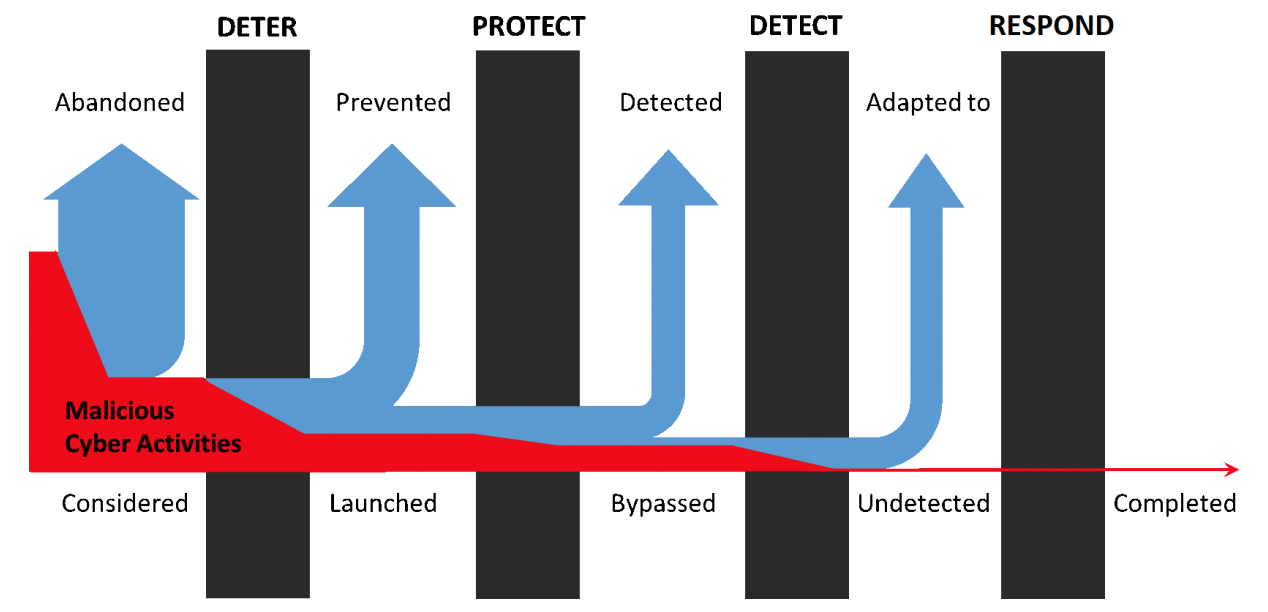
\includegraphics[width=0.9\textwidth]{security_methods.png}
    \caption{应对网络安全攻击的防御手段}
    \label{fig:security_methods}
  \end{figure}

  然而,现有的互联网体系结构并不能很好地对网络攻击实施有效保护,更难以谈及有力的威慑。主要原因在于现在的网络体系结构中,在转发网络数据包时,仅仅关注于根据目的IP地址进行数据包的转发,而不对数据包源IP地址的真实性进行检查。著名的STRIDE威胁模型\cite{kohnfelder1999threats}指出,网络安全问题层出不穷的根源在于源地址的伪造和难以溯源。缺乏对源IP地址真实性的验证机制使得伪造源IP地址的网络攻击流量在转发途中不受任何阻碍,即使能够在攻击对象的那一端对其进行阻止,也足以对网络带宽造成巨大的损耗,占用网络中转发其他正常流量的资源,从而影响网络整体的效益。此外,由于源IP地址不具备真实性的保证,同时IP地址又具有动态配置的特性,与现实世界中的用户实体不相关联,当网络攻击行为发生并被检测到时,人们仅能针对攻击流量进行一定程度的防御,而无法根据其源IP地址追溯到现实世界中的攻击者身份,令其为攻击行为所造成的危害负责,因而极大地损失了对攻击者的威慑力,导致威慑这第一步防御手段形同虚设。

  因此,现有的网络体系结构需要首先解决网络源IP地址伪造的问题,然后在源地址真实的前提下进行IP地址与用户身份的绑定、实现对用户真实身份的溯源功能,从而提供阻断攻击者恶意伪造流量的有效防御手段,并通过有力的审计和追责机制对攻击者形成强烈的威慑。

  针对IP源地址伪造的问题,源地址验证体系结构(Source Address Validation Architecture, SAVA)\cite{RFC5210}提出将互联网划分为接入子网、自治域内和自治域间三个层次,在每个层次分别研究相应的真实源地址验证技术,为源地址伪造的问题提供体系化的解决方案。源地址验证技术的研究,将从体系结构的角度提高网络空间整体的可信性,从根源上杜绝网络空间安全问题的发生,避免网络安全传统研究思路的补丁式解决方案。

  在源地址真实的基础上,充分利用IPv6地址空间巨大的优势,结合用户访问网络时的身份认证手段,通过将网络空间中的IPv6地址与现实世界中的用户身份相绑定的方式,设计实现并推广部署用户身份识别与溯源系统,将解决恶意网络行为责任人的溯源问题,提高对网络行为的精细化管控能力。

  在用户身份识别与溯源系统推广至多个管理域进行大规模部署时,还将面临跨管理域的用户身份溯源问题。由于涉及到用户隐私,因此用户身份溯源的权限必须谨慎地集中控制,而集中式的系统设计又难以抵御数据篡改与拒绝服务攻击,并且引入额外的信任成本。在消除集中式的可信第三方、提升系统可用性与提供数据保护方面,一种叫做区块链(Blockchain)的技术提供了新的解决方案,在近年来引发了人们的广泛关注。其最初作为底层的数据存储技术诞生于比特币(Bitcoin)\cite{nakamoto2019bitcoin}这一虚拟货币之中,但随即由于其去中心化和不可篡改的特性引发了人们的关注,在解决各个行业的一些传统痛点问题方面被寄予厚望。针对比特币协议合约脚本难以扩展的问题而提出的以太坊\cite{wood2014ethereum}与超级账本技术\cite{dhillon2017hyperledger},提供了执行用户自定义合约的能力,使得区块链在实现许多传统软件应用功能的同时,又提供了状态的多副本备份和不可篡改的特性,能够有效提升系统的可用性和安全性,因此吸引了大量的开发者利用区块链构建自己的分布式应用,并被广泛尝试应用于加密货币、金融资产结算、数字政务、防伪存证、物流溯源等多个交叉领域,形成了繁荣的生态。

  \section{论文研究工作与意义}
  \label{introduction:work}
  在传统的网络用户接入场景中,为了对用户上网行为实施精细化管控,并提供一定程度的用户身份审计功能,网络管理者往往通过在网络中实施接入认证的方式获取用户身份,并将用户身份与分配给该用户的IP地址形成绑定关系存在数据库中。但是,在网络中缺乏对源地址保护的情况下,即使进行了IP地址与用户身份的绑定,恶意用户仍可以轻易地伪造IP地址进行网络访问,从而逃避溯源与追责,甚至将恶意行为责任转嫁给其他用户。

  因此,基于IPv6源地址验证技术,在保证地址真实的基础上,研究用户身份识别与溯源技术,更具有现实意义。其与SAVA的源地址验证体系结构关系如图\ref{fig:SAVA_architecture}所示:
  \begin{figure}[ht]
    \centering
    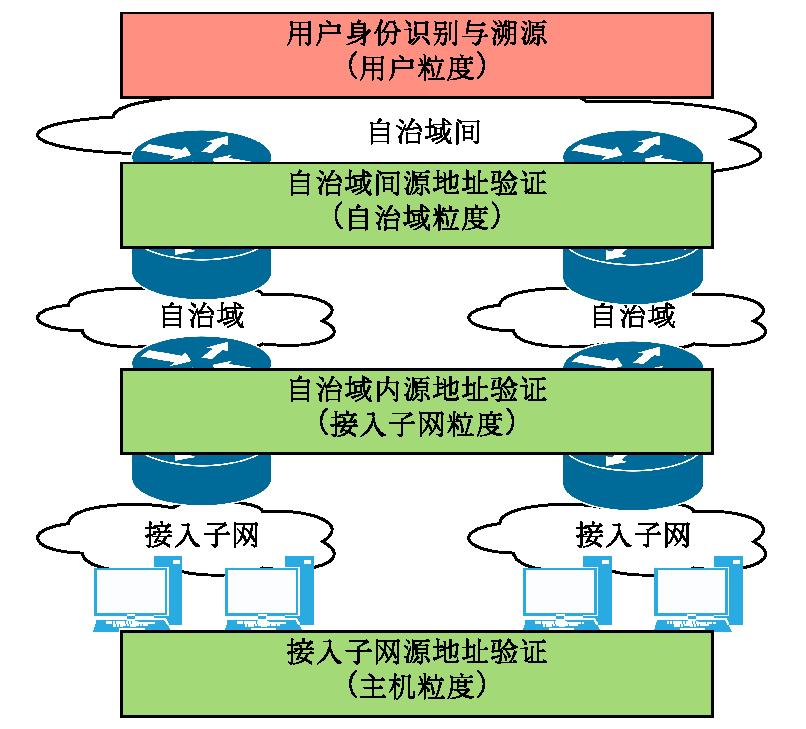
\includegraphics[width=0.7\textwidth]{SAVA_architecture.pdf}
    \caption{用户身份识别与溯源技术研究体系结构}
    \label{fig:SAVA_architecture}
  \end{figure}

  \begin{itemize}
    \item \textbf{接入子网源地址验证}:主机粒度的伪造源地址报文过滤是实现用户身份识别与溯源技术的前提,只有在接入子网内任意用户均只能使用自己真实的IPv6地址访问网络的情况下,最上层基于IPv6地址进行用户身份溯源的技术才不会发生失效或错误溯源的问题。目前接入子网源地址验证的SAVI技术\cite{RFC6959,RFC7039,RFC6620,RFC7513,RFC7219,I-D.bi-savi-wlan}已在IETF基本全部完成标准化,华为、新华三等设备厂商也对其进行了实现与支持,但要实现接入子网内完全的地址防伪造能力,必须在第一跳接入交换机或AP处进行SAVI的全部署,这对于使用目前尚未支持SAVI技术的厂商设备或老旧版本设备的大量接入子网而言,可能存在高昂的替换升级成本,为在接入子网内实现完全的源地址真实造成了一定阻力。
    \item \textbf{自治域内源地址验证}:在自治域内这一层次,由于域内各接入子网的网络均处于同一个管理域的管辖之下,在组网时网络管理员也可以容易地对各接入子网的IP前缀配置过滤规则,因此域内的源地址伪造问题相对而言并不严重,也容易通过一些配置手段加以解决。
    \item \textbf{自治域间源地址验证}:在自治域间发生的源地址伪造,可能导致合法用户遭到恶意用户的跨域伪造,使得用户身份识别与溯源发生错误。由于各自治域有着各自不同的利益考量,部署对自身出域报文的源地址进行验证的技术往往徒增运维负担,而难以带来收益,因此自治域间常需要结成互相信任的安全联盟以进行协作,增加域间源地址验证技术的部署收益。但加入安全联盟的自治域需要依赖于一个可信第三方维护自治域间的互信关系、记录各自治域控制平面通信所需信息,一旦该依赖遭到攻击导致服务不可用或数据篡改,将影响所有自治域间报文的转发,存在着严重的安全隐患。
  \end{itemize}


  即使在源地址得到真实性验证的前提下,传统网络管理中IP地址与身份绑定以实现用户身份溯源这种方式仍存在以下问题:
  \begin{itemize}
    \item \textbf{绑定关系错误}:IP地址的时分复用以及采用NAT技术将多个用户映射至同一个IP地址的不同端口易导致IP地址绑定到错误用户的情况,同时追溯用户时需要确定分组的时间信息,为身份溯源带来困难。
    \item \textbf{存储开销巨大}:为了实现对过去时刻的用户身份追溯,必须将历史上用户接入后的所有绑定关系均保存下来,这在用户时常切换、IP地址分配关系时常变更的网络中常常是难以承受的存储开销。
    \item \textbf{追溯过程复杂}:在互联网中存在数以万计的管理域,对网络攻击行为进行审计的实体与管理该网络攻击行为来源地网络的实体往往来自不同的管理域,多管理域中用户溯源技术不统一以及管理域间的线下协同工作容易引发追溯审计的困难。
    \item \textbf{认证手段限定}:目前广泛实施的IP地址与用户身份绑定都要求在Web Portal认证的方式下进行,其限定了用户认证方式,在无线网络中对终端漫游的支持较差,并且不具备良好的推广性,难以支持二层准入认证的网络环境。
  \end{itemize}

  NIDTGA(Network Identity and Timestamp Generation Address)地址生成方案\cite{liu2015building}针对上述问题,设计了一种通用的用户网络身份标识(Network Identity,NID),并利用IPv6广大地址空间的优势,采取了将NID与用户接入时间进行对称加密后嵌入IPv6的方式为用户生成和分配一种特定的IPv6地址,从而在保护用户隐私的同时将用户身份与IPv6地址实现了强绑定。由于NID结构的通用性,NIDTGA地址生成方案可以适用于用户数量不同的各类管理域。NIDTGA地址加密生成的方式,保证了审计方只需要持有用于生成地址时对称加密的密钥,即可追溯获得标识了用户身份的NID以及用户接入网络的时间,避免了巨大的用户信息绑定的存储开销和复杂的追溯过程。同时,由于嵌入了用户认证上网的时间信息并采用加密方式生成地址,基本消除了IPv6地址的混用情况,用户身份与IPv6地址的绑定错误也被良好避免。

  但是,尽管NIDTGA地址生成方案在理论上解决了传统网络中用户上网行为管理和审计的困难,但其仅给出了NID与NIDTGA地址的设计与生成方法,将用户的上网过程理想化为先提交NID完成认证、后获取NIDTGA地址这样两个简单的步骤,采用其生成算法的用户身份识别与溯源系统仍需要根据实际网络环境进行具体的设计。事实上,用户身份的获取是网络中认证系统的功能,IPv6地址配置是用户设备与相关的IPv6地址配置系统的功能,NIDTGA地址生成方案由于将用户身份与IPv6地址相关联,要求认证系统与IPv6地址配置系统之间实现信息同步的机制,而实际的接入子网环境错综复杂,不仅有着各异的组网方式,还存在着多种广泛应用的认证系统与IPv6地址配置系统,任意一个因素的变化都将影响到用户身份识别与溯源系统的设计:
  \begin{itemize}
    \item \textbf{地址配置方式}:IPv6地址引入了无状态地址自动配置SLAAC协议,其由用户设备自行生成地址而非向一个集中式的服务器进行请求,不存在类似于DHCPv6服务器这样能够控制用户设备配置某个特定IPv6地址的集中控制点,SLAAC与DHCPv6这两者的差异将直接导致各自地址配置方式下用户身份识别与溯源系统的不同设计方案。
    \item \textbf{用户认证手段}:实际网络中得到广泛应用的认证手段多种多样。以网络层为界,常用于在链路层认证的有802.1X\cite{ieee802ieee}、PPPoE\cite{RFC2516}等协议,基于网络层往上进行用户认证控制的则有Web Portal认证、IPoE与Web Portal的组合认证等方式。是否基于网络层协议进行用户身份认证决定了IPv6地址配置过程发生在用户认证前还是认证之后,因此用户身份识别与溯源系统需要根据网络中具体的认证手段对其NIDTGA地址配置流程做出相应的设计。
    \item \textbf{设备类型}:不同厂商的设备对于地址配置方式的支持情况不同,使用Android、Chrome OS等Google系操作系统的用户设备目前不支持DHCPv6配置地址。此外,网络中不止包含普通的笔记本或手机终端,还包括服务器、嵌入式设备等难以进行身份认证的设备。设备类型的繁杂为用户身份识别与溯源系统实现设备全覆盖带来了挑战。
    \item \textbf{子网组网方式}:接入子网根据用户接入方式的不同,可分为有线子网与无线子网,两者对源地址验证技术的部署要求不同,源地址验证设备位置、子网网关位置、以及DHCPv6配置时DHCPv6中继设备位置也不相同。在无线子网配置时,若数据报文直接经由上层有线网络转发,则称为本地转发模式,若全部经由IP隧道到达AC后统一转发,则称为集中转发模式,两种转发模式下数据报文转发路径的不同将影响接入子网中网络设备的配置,同样也影响到用户身份识别与溯源系统的部署方案。
  \end{itemize}

  可见,用户设备如何在获取地址前进行身份认证、如何标识用户设备并将NIDTGA地址与其准确关联、如何在实际的复杂网络环境中进行部署等均是用户身份识别与溯源系统在设计与实现时需要考虑的重要问题。用户身份识别与溯源技术在利用NIDTGA的地址生成理论后,面向实际网络进行系统设计、实现与部署落地等方面还面临着巨大的挑战。

  本文根据上述分析,主要在三个方面开展研究工作:
  \begin{enumerate}[1{)}]
    \item \textbf{接入子网与自治域间源地址验证技术的增强方案。}

    SAVI技术在接入子网范围内进行源地址伪造报文的过滤,其功能的正确行使依赖于网络中各台设备对SAVI的支持与配置情况,其作为较新的国际标准尚未被所有厂商设备良好支持,如何在非理想的SAVI部署网络中进行接入子网源地址伪造的预防有待研究。另一方面,一类重要的自治域间源地址验证技术在方案设计上存在着共同的安全缺陷,其引入的安全联盟概念虽在一定程度上增加了方案的部署激励,但也为域间源地址验证系统的运作带来了单一故障点的安全风险。本文针对上述问题,分别研究采用传统网络设备普遍支持的其他机制配合SAVI技术以较小的代价实现接入子网源地址验证,以及利用区块链构建域间源地址验证方案中的安全联盟,在接入子网为用户身份识别与溯源系统的部署提供有力的源地址真实性保证,并为自治域间保障源地址真实消除重大的安全隐患,为用户身份识别与溯源系统的设计、应用与推广奠定良好的技术基础。

    \item \textbf{各类网络场景下用户身份识别与溯源系统的设计与实现。}

    NIDTGA地址生成方案提出以来,将其应用至实际的用户身份识别与溯源系统仍有待研究。在设计采用NIDTGA地址生成方案的用户身份识别与溯源系统时,由于系统工作于网络层而非仅仅在于应用层,其难以独立于网络环境采用的底层协议而实现统一设计,多种IPv6地址的配置方式、各类用户身份认证手段、不同厂商品牌型号的用户设备均会对用户身份识别与溯源的过程产生影响,因此具备应用推广意义的用户身份识别与溯源技术必须实现对多场景全用户的适配,提出各类网络环境中的用户身份识别与溯源系统设计方案与部署方案。本文首先调研了IPv6地址配置方式,并分析了实际网络中常见的用户认证手段、用户设备对各类地址配置协议与认证手段的支持情况,以确认用户身份识别与溯源系统需要覆盖的网络场景。然后分别针对各种常见地址配置方式与用户身份认证手段的组合,研究系统的设计方案。最后本文还调研了全国主要高校的组网情况,以常见的校园网环境为例,讨论了对用户身份识别与溯源系统进行推广时的网络设备支持要求,总结抽象出部署方案的指导框架。

    \item \textbf{基于区块链的跨管理域用户身份溯源系统设计与实现。}

    在用户身份识别与溯源系统推广部署的过程中,需要解决跨管理域的用户身份溯源问题。由于溯源过程涉及用户身份隐私,因此用户溯源权限必须谨慎地进行集中控制。但如果采用集中式的组织密钥历史存储与用户身份溯源,则存在中心化的安全风险,易受到恶意攻击,引发服务不可用或数据篡改,从而导致用户隐私泄露与溯源功能失效。如何多副本备份组织密钥历史并对其实施有效的数据保护,但仍集中地控制用户身份溯源权限,避免用户隐私泄漏,是跨管理域的用户身份溯源系统亟待解决的问题。本文研究将区块链应用于构建用户身份溯源系统的设计方案,利用区块链分布式的优势保证各组织密钥历史的多副本备份,利用其数据不可篡改的特性保证密钥历史的真实性,并且使用椭圆曲线加密算法加密密钥历史,以确保在数据对各个区块链节点可见的情况下仍只有审计方有能力读取各组织的密钥历史明文。

  \end{enumerate}


  \section{论文贡献}
  \label{introduction:contribution}
  本文的主要贡献包括:
  \begin{enumerate}[1{)}]
    \item 针对接入子网与自治域间源地址验证技术面临的安全问题,提出了基于VLAN划分的SAVI技术部署增强方案与基于区块链的安全联盟增强方案RegChain,分别解决了非理想的SAVI部署网络环境中的接入子网源地址伪造问题、自治域间SMA方案的单一故障点问题,为用户身份识别与溯源系统奠定良好的源地址真实性保障基础。
    \item 针对网络中用户身份识别与溯源能力的缺乏,提出了采用NIDTGA地址生成方案的用户身份识别与溯源系统,并给出了在各类地址配置方式、用户认证手段组合下的系统设计,提供了覆盖复杂的接入网络全场景的完备解决方案,并对各方案的优缺点进行了评价对比,给出了适宜推广的基于二次准入认证的系统在校园网络中的部署方案。
    \item 对各类网络场景下的用户身份识别与溯源系统设计进行了实现、测试与部署,其中DHCPv6配置下基于二次准入认证的系统已在清华大学无线校园网络中得到部署并计划在全国主要高校进行推广,基于扩展DHCPv6协议认证的系统已在清华、北大等5所高校进行了部署实验,并通过了国家发改委288项目的验收。在SLAAC下的用户身份识别与溯源技术基础上,增加了对MAC地址伪造的检测与预防的溯源方案已由华为和新华三厂商进行实现,并开始在清华大学无线网络中进行大规模部署与应用。
    \item 针对用户身份识别与溯源系统推广部署时的跨管理域溯源问题,提出溯源系统的区块链设计方案NIDChain,在提供数据安全与服务高可用优势的同时,设计了相应的权限控制机制确保用户身份溯源权限高度集中,为用户身份识别与溯源系统的大规模部署奠定了基础。
  \end{enumerate}


  \section{论文组织结构}
  \label{introduction:structure}
  本文共分六章,各章节之间的逻辑关系如图\ref{fig:thesis_structure}所示,具体组织如下:
  
  第一章为论文引言,主要介绍IPv6源地址验证与用户身份识别与溯源技术的背景、研究工作与意义以及论文对用户身份识别与溯源相关技术的贡献。

  第二章为论文相关研究工作的综述,主要介绍了IPv6地址的几种配置协议、源地址验证各个层次的相关技术、IPv6地址生成方案、现有的用户身份识别与溯源方案以及区块链的相关研究。
  
  第三章为论文研究的第一部分,IPv6源地址验证技术的增强方案,从接入子网与自治域间两个层次分别介绍了基于VLAN划分的SAVI部署增强方案与基于区块链的安全联盟增强方案RegChain。

  第四章为论文研究的第二部分,用户身份识别与溯源系统的设计、实现与部署。首先分析了用户身份识别与溯源系统需要支持的复杂网络场景,然后针对DHCPv6、SLAAC与静态地址三种地址配置方式下基于Web Portal、二层准入认证等不同用户认证手段的系统设计方案进行研究与实现,介绍了目前各场景下用户身份识别与溯源系统的应用现状,分析了各种设计方案的优劣性,并给出了在校园网络中部署应用的指南。

  第五章为论文研究的第三部分,基于区块链的用户身份溯源系统研究。提出了利用区块链构建跨管理域的溯源系统设计方案NIDChain,探讨了在区块链上所有数据公开透明的情况下确保各组织密钥历史的私密性并赋予审计方唯一追溯权限的机制,详细介绍了智能合约中密钥历史更新等各个功能的设计,并基于以太坊进行了实现。

  第六章对全文的工作进行了总结,并展望了后续推进用户身份识别与溯源技术的研究方向。

  \begin{figure}[ht]
    \centering
    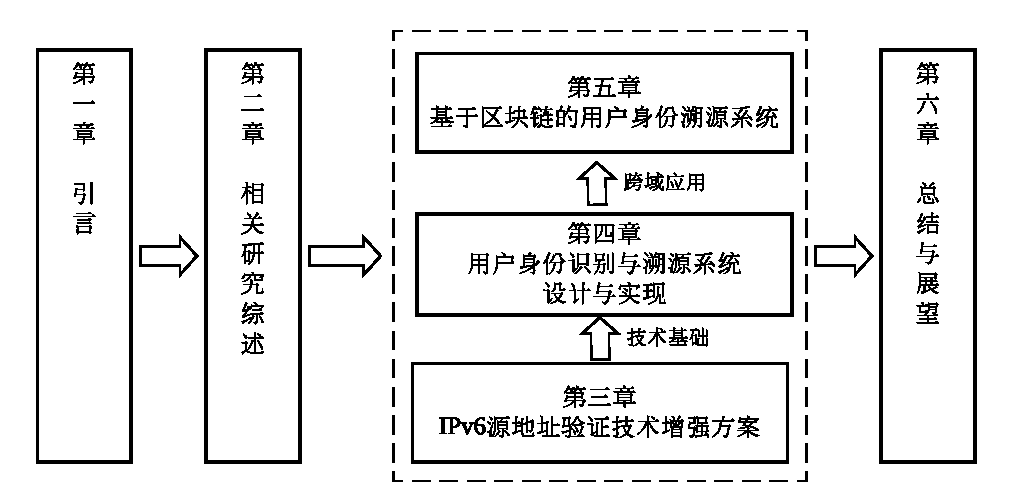
\includegraphics[width=0.9\textwidth]{thesis_structure.pdf}
    \caption{论文组织结构}
    \label{fig:thesis_structure}
  \end{figure}